\section{Simulation Analysis}
\label{sec:simulation}

In this section, the circuit shown in Figure~\ref{fig:rc} is simulated with the use of NGSpice. Using the operating point analysis for both $t<0~s$ and $t=0~s$, we determine the initial conditions needed for the transient analysis, which in turn simulates the circuit's total response.
Because of the use of NGSpice for this simulation, there was a need to create a "dummy" voltage source, between nodes 7 and 8, that provided $0~V$ to the circuit (thus not changing the behavior of the original circuit). Because this is just a technical issue that does not affect the original circuit, the one shown in Figure~\ref{fig:rc} can be used for illustrative purposes.


\subsection{Operating Point Analysis}

Table~\ref{tab:op} shows the simulated operating point results for $t<0~s$, where it's assumed that no current flows through the capacitor (open circuit).
Table~\ref{tab:op2} shows the simulated operating point results for $t=0~s$, where $V_S$ is short-circuited and the capacitor is replaced with a voltage source $V_x = V(6) - V(8)$ (with $V(6)$ and $V(8)$ as obtained in Table~\ref{tab:op}.


\begin{table}[h]
	\parbox{.45\linewidth}{
  \centering
  \begin{tabular}{|l|r|}
    \hline    
    {\bf Name} & {\bf Value [A or V]} \\ \hline
    v(1) & 5.048640e+00\\ \hline
v(2) & 4.860629e+00\\ \hline
v(3) & 4.468710e+00\\ \hline
v(4) & 4.888344e+00\\ \hline
v(5) & 8.679973e+00\\ \hline
v(6) & -2.02627e+00\\ \hline
v(7) & -3.01571e+00\\ \hline
v(8) & -3.01571e+00\\ \hline

  \end{tabular}
  \caption{Operating point data for $t<0~s$. A variable preceded by @ is of type Current and is expressed in Ampere; other variables are of type Voltage and are expressed in Volt.}
  \label{tab:op}
}
\hfill
	\parbox{.45\linewidth}{
  \centering
  \begin{tabular}{|l|r|}
    \hline    
    {\bf Name} & {\bf Value [A or V]} \\ \hline
    v(1) & 5.048640e+00\\ \hline
v(2) & 4.860629e+00\\ \hline
v(3) & 4.468710e+00\\ \hline
v(4) & 4.888344e+00\\ \hline
v(5) & 8.679973e+00\\ \hline
v(6) & -2.02627e+00\\ \hline
v(7) & -3.01571e+00\\ \hline
v(8) & -3.01571e+00\\ \hline

  \end{tabular}
  \caption{Operating point data for $t=0~s$. A variable preceded by @ is of type Current and is expressed in Ampere; other variables are of type Voltage and are expressed in Volt.}
  \label{tab:op2}
}	
\end{table}
            

\par Compared to the theoretical analysis results, one notices that the simulated data matches almost perfectly the theoretical values. This is expected, as the circuits being simulated in both scenarios are exclusively composed by linear components. Moreover, the slight discrepancies (of the order of $1e-15$) can be associated to the precision of ngspice and to some approximations made by octave because of the precision of the floating point used.

\newpage
\subsection{Transient Analysis}

\subsubsection{Natural Response}

Figure~\ref{fig:trans} shows the plot of the simulated transient analysis results in the interval $[0, 20]~ms$, using the boundary conditions of $V(6)$ and $V(8)$ as determined before. 
Once again, the simulation data matches with the theoretical natural response prediction, and one can clearly see the negative exponential behavior of $V(6)$, as was expected.

\begin{figure}[h] \centering
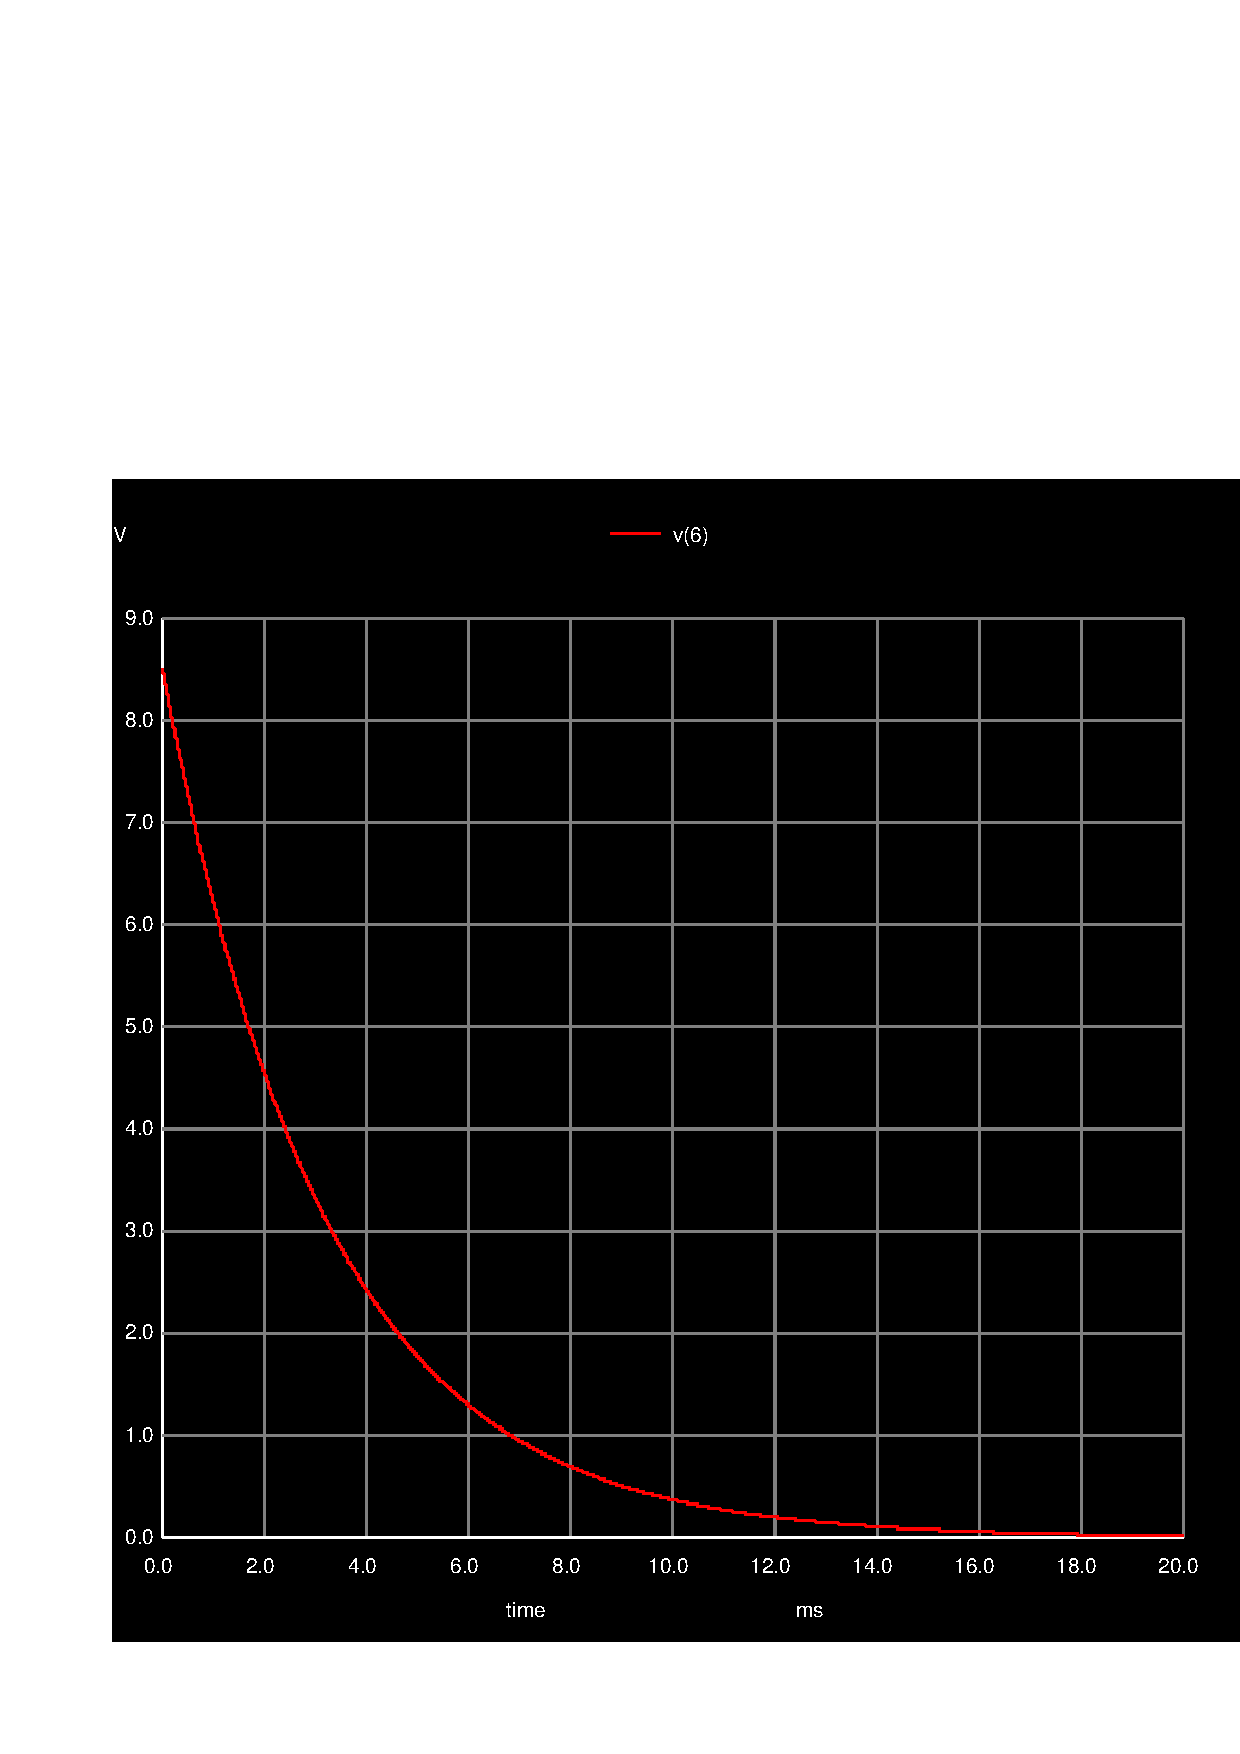
\includegraphics[width=0.6\linewidth]{natural.pdf}
\caption{Natural response of $V_{6}$ in the interval $[0, 20]~ms$.}
\label{fig:trans}
\end{figure}

\newpage

\subsubsection{Total Response}

Figure~\ref{fig:totalsim} shows the plot of the simulated transient analysis results in the interval $[0, 20]~ms$, by using $V_S(t)$ as given in Figure~\ref{fig:rc} and $f = 1~kHz$. 
Once again, the simulation data matches with the theoretical total response prediction, as was expected.
                                    

\begin{figure}[h] \centering
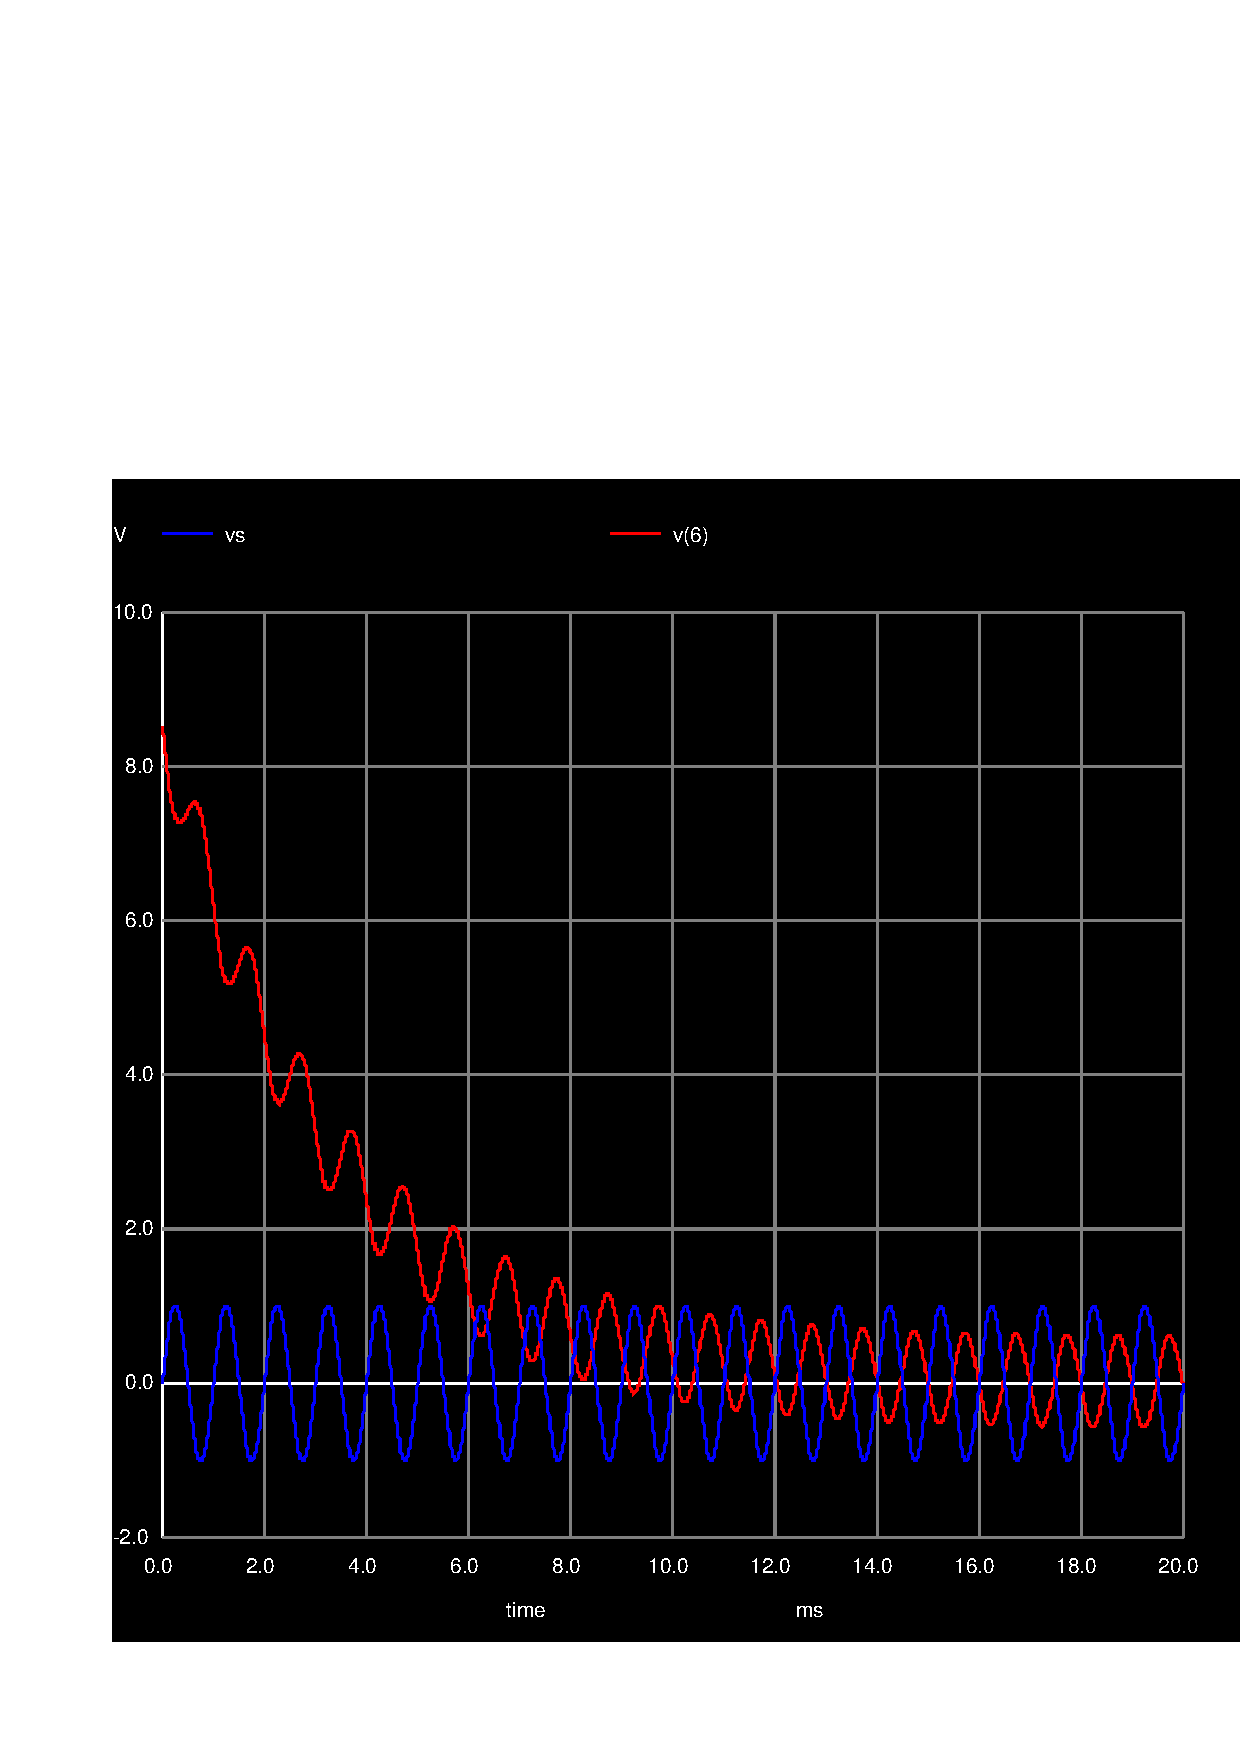
\includegraphics[width=0.6\linewidth]{total.pdf}
\caption{Total response of $V_{6}$ and $V_S$ in the interval $[0, 20]~ms$.}
\label{fig:totalsim}
\end{figure}

\newpage

\subsection{Frequency Analysis}

In this section, the frequency response in node 6 is simulated, with the frequency in logscale, magnitude in $dB$ and phase in $degrees$, for the frequency range of $0.1~Hz$ to $1~MHz$.


\subsubsection{Magnitude Response}

Figure~\ref{fig:magsim} shows the magnitude of the frequency response for the circuit under analysis. Compared to the theoretical analysis results, one notices a clear match between plots. Thus, the reasons for how $V(6)$ and $V_S$ differ from each other are the same as explained in the theoretical analysis above.

\begin{figure}[h] \centering
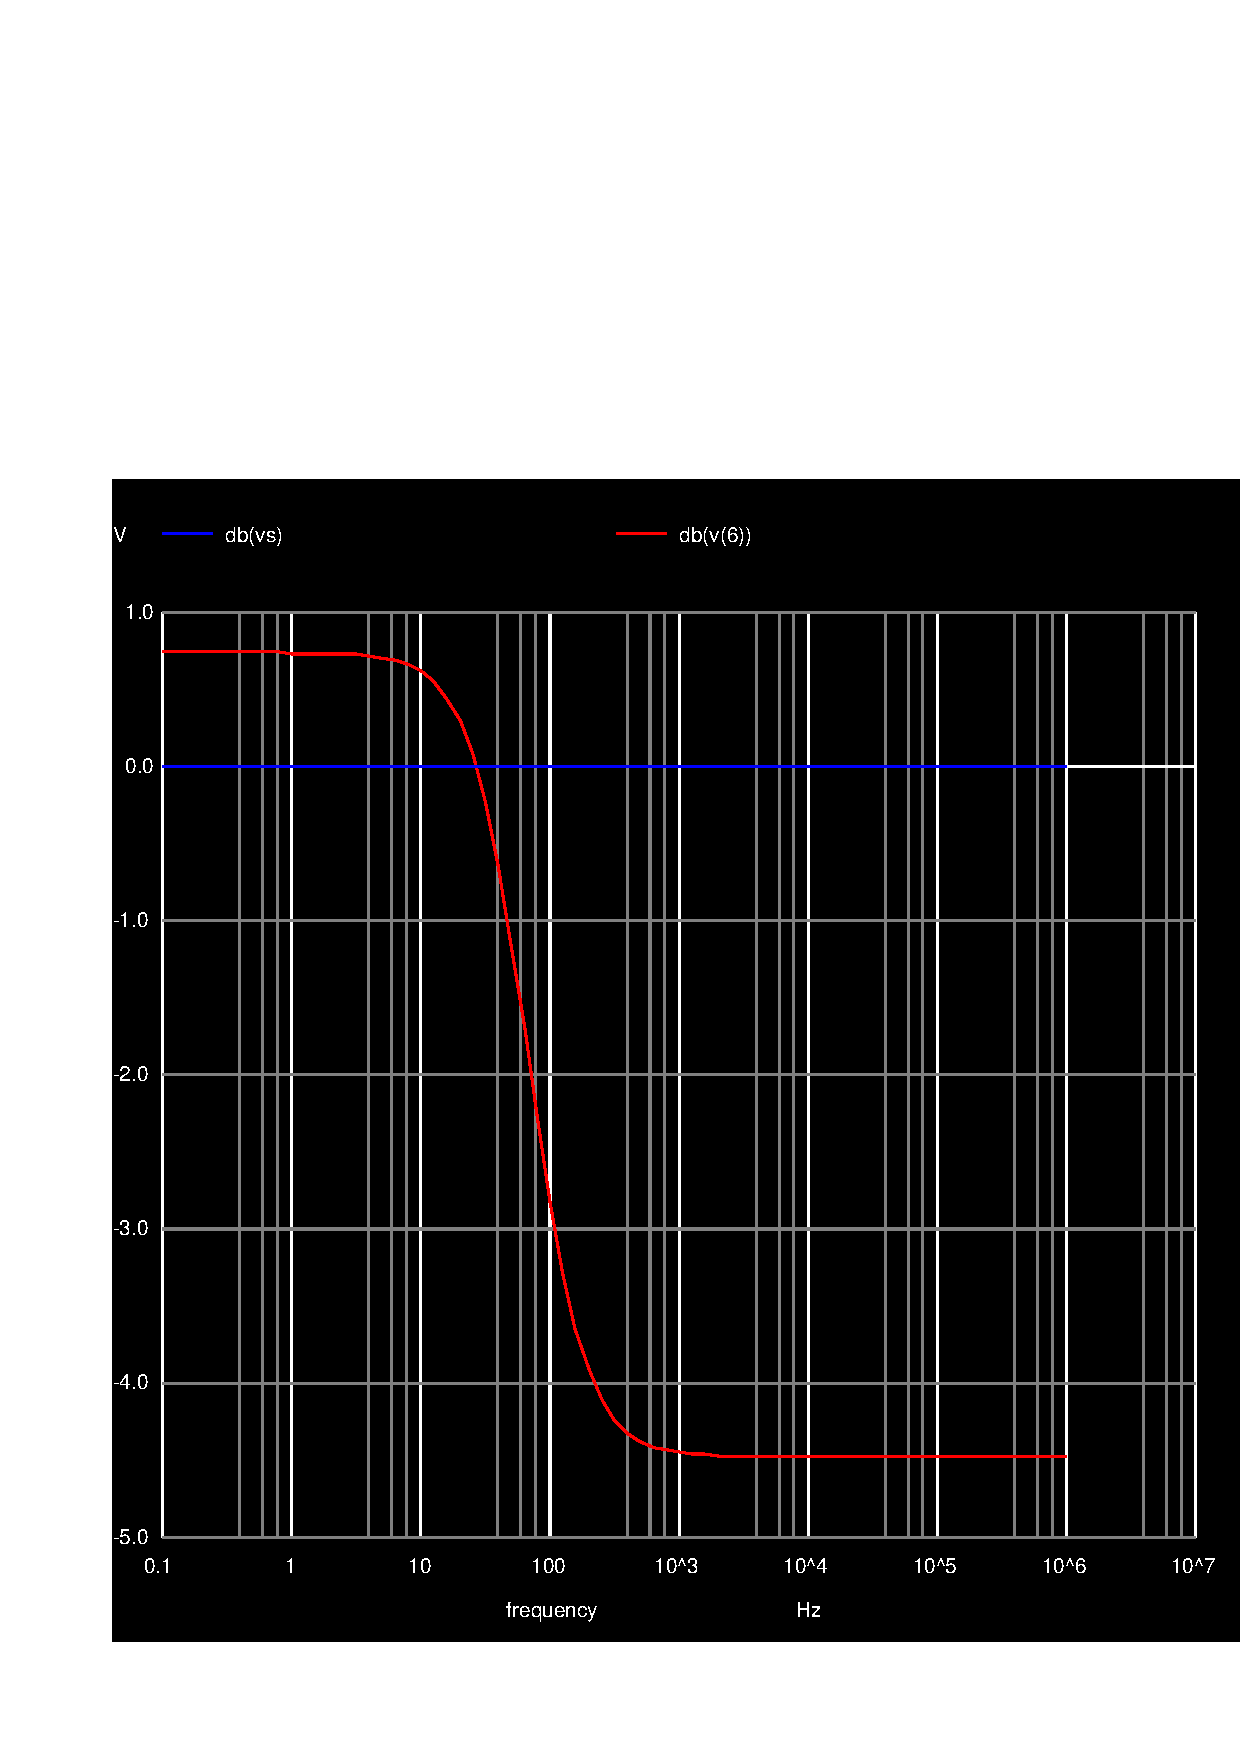
\includegraphics[width=0.6\linewidth]{magnitude.pdf}
	\caption{Magnitude of frequency response of $V(6)$ and $V_S$ plot.}
\label{fig:magsim}
\end{figure}

\newpage

\subsubsection{Phase Response}

Figure~\ref{fig:phasesim} shows the magnitude of the frequency response for the circuit under analysis. Compared to the theoretical analysis results, one notices a clear match between plots. Thus, the reasons for how $V(6)$ and $V_S$ differ from each other are the same as explained in the theoretical analysis above.

\begin{figure}[h] \centering
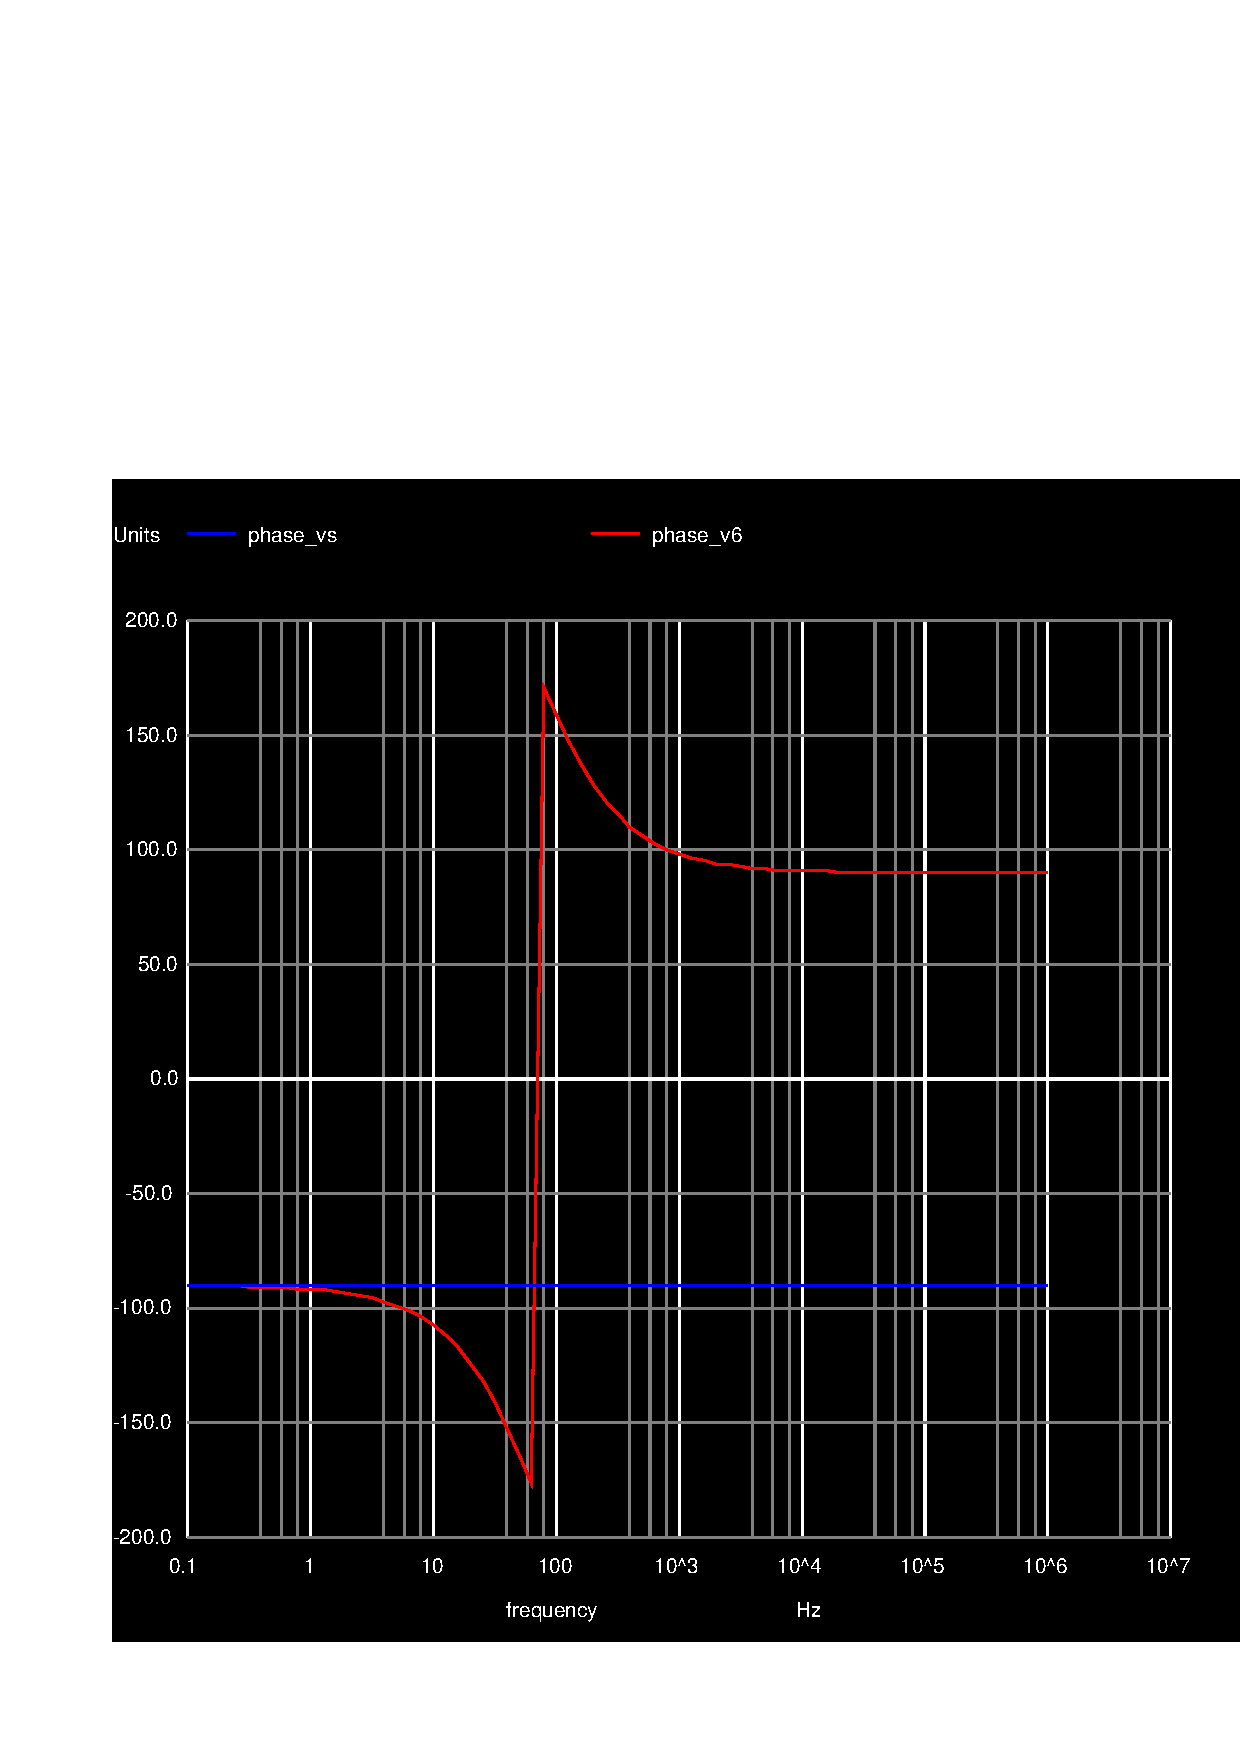
\includegraphics[width=0.6\linewidth]{phase.pdf}
	\caption{Phase response of $V(6)$ and $V_S$ plot.}
\label{fig:phasesim}
\end{figure}

